%\documentclass[preprint, review, 3p, authoryear]{elsarticle}
\documentclass[10pt, a4paper]{article}

%\usepackage{setspace}
\usepackage[utf8]{inputenc}
\usepackage{amsmath, amssymb, amsthm, bbm}
\usepackage{xcolor}
\usepackage{graphicx}
\usepackage[authoryear]{natbib}
\usepackage{apalike}
\usepackage{relsize}
\usepackage{array}
\usepackage{multirow}
\usepackage{showlabels}
\usepackage{setspace}
\usepackage[normalem]{ulem}
\usepackage{xspace}
%Add line numbering
%Line numbering can be incorporated by using the lineno package. Add these statements in the preamble:
\usepackage{lineno}
\linenumbers

\DeclareMathOperator*{\argmax}{arg\,max}

\newtheorem{prob}{Problem}
\newtheorem{prop}{Proposition}
\newtheorem{definition}{Definition}

%%%%% bold symbol in math enviornment
\newcommand{\m}[1]{\boldsymbol{#1}}

\newcommand{\fmm}{\textsc{fmm}\xspace}

\title{Merging the components of a finite mixture using  posterior probabilities}
\author{M. Comas-Cufí \and J.A. Martín-Fernández \and G. Mateu-Figueras}

%\doublespacing
\begin{document}

\begin{spacing}{1.9}
%%%%%%% BEGIN SPACING


\pagenumbering{arabic}

\maketitle

\section{Introduction}


% Mixture models
A common approach in parametric cluster analysis assumes data can be modelled by means of a \emph{finite mixture of distributions}, also called \emph{finite mixture model} (\fmm). A \fmm is a probability distribution with probability density function (pdf) defined as the linear combination of pdf from distributions with same domain $\mathbb{X}$. In general, the pdf $f$ of a \fmm is
\begin{equation}\label{mixt}
f(\;\cdot\; ; \pi_1, \dots, \pi_k, \m\theta_1, \dots, \m\theta_k) = \pi_1 f_1(\;\cdot\; ; \m\theta_1) + \dots + \pi_k f_k(\;\cdot\; ; \m\theta_k),
\end{equation}
where $\m\theta_1, \dots,  \m\theta_k$ are the parameters of the pdf $f_1, \dots, f_k$ respectively and, because $\int_{\mathbb{X}}f = 1$ the restriction $\sum_{\ell = 1}^k \pi_\ell = 1$ holds. The pdf $f_1, \dots, f_k$ are called the \emph{components} of the \fmm, or simply the \emph{mixture components}. When model-based clustering is based on \fmm's, the clustering approach follows two steps:
\begin{enumerate}
\item to find suitable estimators $\hat{\pi}_1, \dots, \hat{\pi}_k,$ $\hat{\m\theta}_1, \dots, \hat{\m\theta}_k$ of parameters $\pi_1, \dots, \pi_k,$ $\m\theta_1, \dots, \m\theta_k$, and
\item to classify each observation according to the maximum a posteriori criteria, i.e., one observation $\m x_i \in \mathbb{X}$ is classified to cluster $c$ if and only if
\begin{equation}\label{map_criteria}
c=\argmax_{j=1}^k \frac{ \hat{\pi}_j f_j(\m x_i ; \hat{\m\theta}_j) }{\sum_{\ell=1}^k \hat{\pi}_\ell f_\ell(\m x_i ; \hat{\m\theta}_\ell) }.
\end{equation}
\end{enumerate}
Note that in this process, the number of clusters $k$ is fixed in advance. 

\cite{lee2004combining,hennig2010methods,baudry2010combining,melnykov2013distribution,pastore2013merging} noted that associating one mixture component to one cluster can be misleading because different mixture components can be not separated enough to be considered as a unique cluster. Instead, they proposed one cluster could be formed by the combination of different mixture components. Therefore, one crucial point of this clustering method is how to decide which components have to be merged, the focus of this article.


We introduce a generic approach to decide which two components should be merged, the approach we introduce depends on two different functions $\lambda$ and $\omega$ which should be defined a priori. For different choices of this functions our approach contains the proposals given by \cite{baudry2010combining}, the DEMP approach introduced by \cite{hennig2010methods} and \cite{longford2014}. Once the criterion for merging component is adopted, from the initial \fmm we can build a hierarchy over the set of components and see which components are more likely to form a single cluster.

The paper is organised as follows: $\dots$


\section{Definitions and notation}

%
A \emph{partition} of $\{1, \dots, k\}$, $\mathcal{P}_s$,  is a set of subsets $I_p$ of $\{1, \dots, k\}$, $1\leq p \leq s$, called $parts$, such that $\bigcup_{I_p \in \mathcal{P}_s} I_p = \{1, \dots, k\}$ and for any two parts $I_a, I_b \in \mathcal{P}_s$ with $a \neq b$, $I_a \cap I_b = \emptyset$ holds. It is important to note that for any partition  $\mathcal{P}_s$ the pdf $f$ of a \fmm (Eq.~\ref{mixt}) can be rewritten as
\begin{equation}
f = \pi_{I_1} f_{I_1} + \dots + \pi_{I_s} f_{I_s},
\label{mixt_part}
\end{equation}
where $f_{I_p} = \sum_{j \in I_p} \frac{\pi_j}{\pi_{I_p}} f_j(\;\cdot\; ; \m\theta_j)$ and $\pi_{I_p} = \sum_{\ell \in I_p} \pi_\ell$. Moreover, note that using this notation $f_{I_p}$ is also a \fmm.



A \emph{hierarchical sequence of partitions of $\{1,...,k\}$}, is a sequence of partition $\mathcal{P}_1, \dots, \mathcal{P}_k$ verifying that
  
\begin{itemize}
\item $\mathcal{P}_1$ is the one-part partition $\mathcal{P}_1 = \{ \{1, \dots, k\} \}$,
\item for each $s$, $1 <  s \leq k$, $\mathcal{P}_{s}$ has $s$ elements,
\item if a part $I_p \in \mathcal{P}_{s-1}$ then either there is a part $I_a \in \mathcal{P}_{s}$ with $I_p = I_a$ or there are two parts $I_a, I_b \in \mathcal{P}_s$ with $I_p = I_a \cup I_b$, and
\item $\mathcal{P}_k= \{ \{1\},\{2\}, \dots, \{k\} \}$.
\end{itemize}



One can extend Eq.~\ref{map_criteria} in terms of partitions. Indeed, let $\rm X = \{\m x_1,\dots, \m x_n\}$ be a sample defined in $\mathbb{X}$. Given a partition $\mathcal{P}_s = \{ I_1, \dots, I_s \}$ the posterior probability of $\m x_i$ being classified to part $I_p\in \mathcal{P}_{s}$ is
\[
\hat{\tau}_{i I_p} =  \frac{ \hat{\pi}_{I_p} \hat{f}_{I_p}(\m x_i) }{\sum_{\ell=1}^s \hat{\pi}_{I_\ell} \hat{f}_{I_\ell}(\m x_i)}.
\]
where $\hat{\pi}_{I_p} = \sum_{\ell \in I_p} \hat{\pi}_\ell$ and $\hat{f}_{I_p}(\m x_i) = f_{I_p}(\m x_i; \hat{\theta})$. From now on, if there is now confusion with parameter $\hat{\theta}$, we are going to use this simplified notation. 

For the partition  $\mathcal{P}_s$, we define the posterior probability vector as
\[
\hat{\m\tau}_{i \mathcal{P}_s} = \left( \hat{\tau}_{i I_1} , \dots, \hat{\tau}_{i I_s}  \right).
\]
Note that because of $\mathcal{P}_s$ is a partition, $\sum_{p=1}^s \hat{\tau}_{i I_p} = 1$ for $1 \leq i \leq n$.
Moreover, $\m x_i \in \rm X$ is classified to the cluster $c$ if and only if
\begin{equation}\label{cluster_criteria}
c= \argmax_{p=1}^s \{ \hat{\tau}_{i I_p} \}
\end{equation}

\subsection{Example}

Consider following Gaussian mixture with 6 components
\[
\hat{f} = \sum_{j=1}^6 \hat{\pi}_j \phi(\;\cdot\; ; \hat{\m\mu}_j, \hat{\m\Sigma}_j)
\]
and parameters given by
{\small \input{tex/partition-example-pars.tex} }


A random generation of numbers following mixture $\hat{f}$ is represented in Figure~\ref{ex_mixture}. Note that although the finite mixture has 6 components, in the plot 3 clusters are suggested.


\begin{figure}[thbp]
\begin{center}
\begin{tabular}{cc}
 %   6 toy mixture
  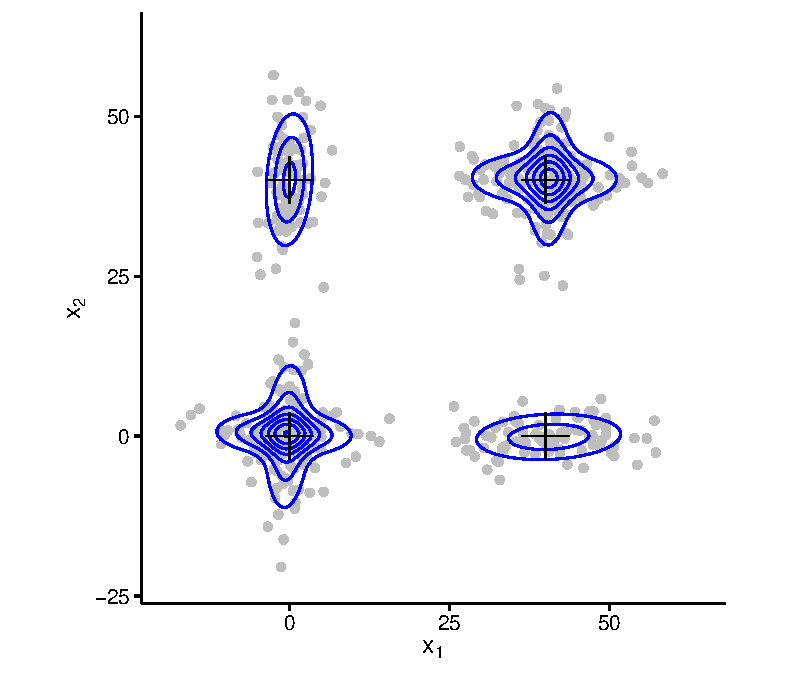
\includegraphics[width=0.7\textwidth]{figures/partition-example-mixture.pdf} \\
 \end{tabular}
 \caption{Density of a Gaussian mixture with 6 component adjusted to a data set generated from a 3 component Gaussian mixture using R \textsc{MixSim} package with max overlapping of $\check{\omega} = 0.01$. Sample mean of each component is represented by '+'.}\label{ex_mixture}
\end{center}
\end{figure}







%%% BIBLIOGRAPHY
\newpage

\bibliographystyle{apalike}
\begin{thebibliography}{}

\bibitem[Aitchison, 1986]{aitchison1986statistical}
Aitchison, J. (1986).
\newblock {\em {The Statistical Analysis of Compositional Data}}.
\newblock Monographs on Statistics and Applied Probability. Chapman \& Hall
  Ltd., London (UK).

\bibitem[Aitchison, 2002]{aitchison2002simplicial}
Aitchison, J. (2002).
\newblock {\em {Simplicial inference}}.
\newblock {\em Algebraic Methods in Statistics anb Probability}, 287: 1--22.

\bibitem[Baudry et~al., 2010]{baudry2010combining}
Baudry, J.-P., Raftery, A.~E., Celeux, G., Lo, K., and Gottardo, R. (2010).
\newblock {Combining Mixture Components for Clustering}.

\bibitem[Hennig, 2010]{hennig2010methods}
Hennig, C. (2010).
\newblock {Methods for merging Gaussian mixture components}.
\newblock {\em Advances in Data Analysis and Classification}, 4(1):3--34.

\bibitem[Lee and Cho, 2004]{lee2004combining}
Lee, H.-j. and Cho, S. (2004).
\newblock {Combining Gaussian Mixture Models}.
\newblock In Yang, Z., Yin, H., and Everson, R., editors, {\em Intelligent Data
  Engineering and Automated Learning – IDEAL 2004 SE - 98}, volume 3177 of
  {\em Lecture Notes in Computer Science}, pages 666--671. Springer Berlin
  Heidelberg.

\bibitem[Longford and Bartosova, 2014]{longford2014}
Longford, N.~T. and Bartosova, J. (2014).
\newblock {A confusion index for measuring separation and clustering}.
\newblock {\em Statistical Modelling}, 14(3):229--255.

\bibitem[Meila, 2006]{meila2006comparing}
Meila, M (2006).
\newblock {Comparing clusterings - an information based distance}.
\newblock {\em Journal of Multivariate Analysis}, 98:873--895.

\bibitem[Melnykov, 2013]{melnykov2013distribution}
Melnykov, V. (2013).
\newblock {On the Distribution of Posterior Probabilities in Finite Mixture
  Models with Application in Clustering}.
\newblock {\em Journal of Multivariate Analysis}, 122:175--189.

\bibitem[Pastore and Tonellato, 2013]{pastore2013merging}
Pastore, A. and Tonellato, S.~F. (2013).
\newblock {A Merging Algorithm for Gaussian Mixture Components}.
\newblock {\em SSRN Electronic Journal}, (04).

\bibitem[Melnykov et~al., 2012]{melnikov2012mixsim}
Melnykov, V. and Chen, W.C. and Maitra, R. (2012).
\newblock {MixSim: An R Package for Simulating Data to Study Performance of Clustering Algorithms}.
\newblock {\em Journal of Statistical Software}, 51(12).

\end{thebibliography}

%%%%%%%%%%% END SPACING
\end{spacing}

\end{document}
